
\documentclass[10pt,a4paper]{article}
\usepackage[margin=1.8cm]{geometry}
\usepackage{booktabs,longtable,array,tabularx,makecell}
\usepackage{amsmath,amssymb}
\usepackage{graphicx,float,placeins}
\usepackage{xcolor,hyperref,url}
\usepackage{enumitem,pdflscape}
\usepackage[T1]{fontenc}
\usepackage{lmodern}
\definecolor{navy}{HTML}{174A6E}
\definecolor{lightblue}{HTML}{E8F1F8}
\definecolor{passgreen}{HTML}{237A3B}
\hypersetup{colorlinks=true,linkcolor=navy,urlcolor=navy}
\setlist{nosep,leftmargin=1.5em}
\renewcommand{\arraystretch}{1.15}
\newcommand{\decision}{\paragraph{Decision.}}
\newcommand{\implementation}{\paragraph{Implementation.}}
\newcommand{\actual}{\paragraph{Actual output.}}
\newcommand{\modelmeaning}{\paragraph{Modeling meaning.}}
\newcommand{\limitation}{\paragraph{Limitation.}}
\title{\textbf{Feature Preparation and Experimental Design Report\\for \texttt{SLURRY\_FREE\_ACID} Forecasting}}
\author{TSP Fertilizer Process Analytics Project}
\date{Executed notebook basis: 16 July 2026}
\begin{document}
\maketitle
\begin{abstract}
This report documents the fully executed \texttt{02\_feature\_engineering\_data\_preparation.ipynb}. The preparation layer now supports four direct forecasting horizons and four hypothesis-driven feature sets. It does not train a predictive model. All numerical claims, tables, and figures in this report are derived from the notebook's exported audit artifacts after a clean, top-to-bottom execution.
\end{abstract}
\tableofcontents
\clearpage

\section{Executive decision and scientific purpose}
The preparation stage is no longer intended to maximize matrix width. Its purpose is to establish a controlled experiment that can test: (1) whether current measurements suffice; (2) whether selected histories add value; (3) whether process relationships improve prediction and interpretation; (4) whether temporal and physical evidence are complementary; and (5) how predictability degrades as warning time increases.

The direct targets are
\[
y_{t+h}=\mathrm{SLURRY\_FREE\_ACID}_{t+h},\qquad h\in\{1,5,10,15\}\ \text{minutes}.
\]
Every input attached to timestamp $t$ uses only measurements available at $t$ or earlier. Feature-set ablation and horizon degradation are therefore first-class experimental questions for the next stage.

\begin{figure}[H]\centering
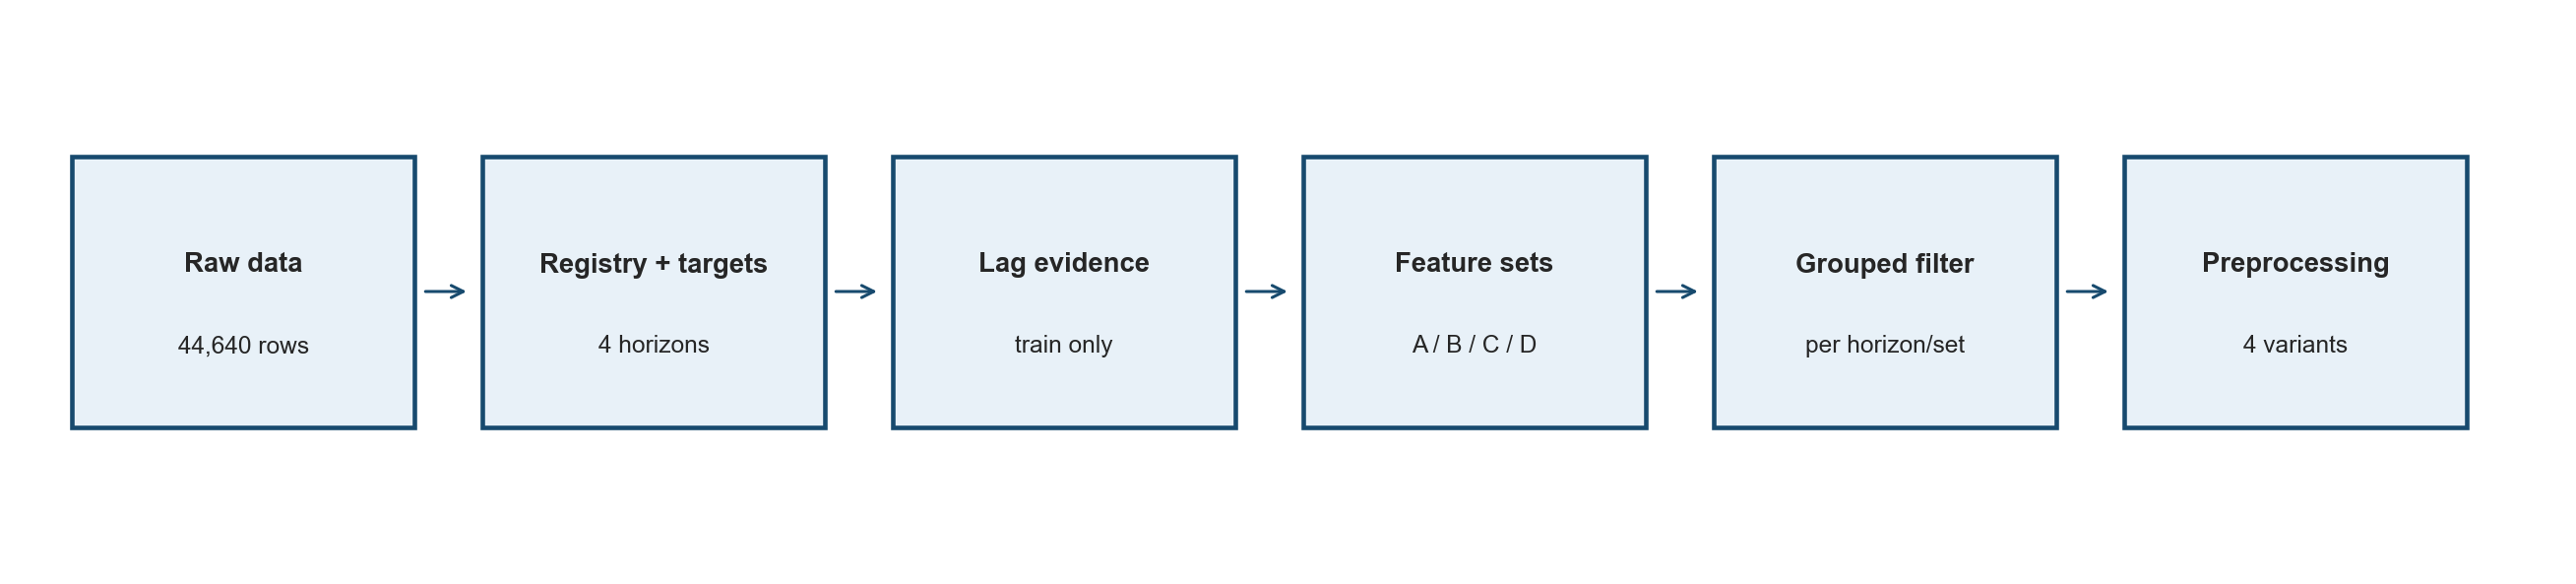
\includegraphics[width=\textwidth]{feature_preparation_artifacts/figures/pipeline_overview.png}
\caption{Executed feature-preparation pipeline.}\end{figure}

\section{Dataset and execution basis}
\decision The notebook uses one chronologically ordered one-minute dataset and excludes the target from the 21 sensor inputs.
\implementation Timestamps are parsed as UTC and sorted before target or feature construction. The notebook was regenerated, executed in a fresh Python process, and saved with execution counts for every code cell.
\actual The execution completed all 11 code cells, exported 21 CSV audit tables and seven figures, and passed all readiness assertions.
\modelmeaning The report is traceable to machine-readable artifacts rather than copied source-code intentions.
\limitation A complete month is available, but one month cannot establish seasonal, campaign, or product-grade robustness.


\begin{table}[H]
\centering
\small
\begin{tabular}{p{0.31\textwidth}p{0.62\textwidth}}
\toprule
Item & Executed value \\
\midrule
Source & \nolinkurl{tsp_1min.csv} \\
Raw rows & 44,640 \\
Input sensors & 21 \\
Missing target observations & 308 \\
Timestamp range & 2026-01-01 00:00:00+00:00 to 2026-01-31 23:59:00+00:00 \\
Sampling / coverage & 1 minute; 31 days \\
\bottomrule
\end{tabular}
\caption{Dataset and timestamp summary.}\label{tab:dataset}
\end{table}


\section{Process-variable registry and intervention safety}
\decision Every source variable is registered before engineering, with a primary category, category tags, role, controllability status, measurement type, physical interpretation, interpretation status, unit-validation status, and recommendation flag.
\implementation Candidate actuator tags are labelled \texttt{needs\_supervisor\_confirmation}; they are not silently promoted to controllable. \texttt{recommendation\_allowed} becomes true only for \texttt{confirmed\_controllable} variables.
\actual No variable is currently confirmed controllable and no change recommendation is authorized. Units are not supplied by the source CSV. Two tags have uncertain roles and two flow-related interpretations require process confirmation.
\modelmeaning The registry supports grouping, explanations, scenario design, and a hard safety boundary between observed state and authorized intervention.
\limitation Registry entries are engineering hypotheses until tag dictionaries, units, locations, and actuator authority are reviewed by the supervisor.


\begin{table}[H]
\centering
\small
\begin{tabular}{p{0.25\textwidth}p{0.48\textwidth}r}
\toprule
Primary category & Role & Variables \\
\midrule
\nolinkurl{flow} & \nolinkurl{candidate_actuator_not_confirmed} & 6 \\
\nolinkurl{flow} & \nolinkurl{observed_state} & 3 \\
\nolinkurl{observed_state} & \nolinkurl{observed_state} & 1 \\
\nolinkurl{possible_quality_indicator} & \nolinkurl{target} & 1 \\
\nolinkurl{pressure} & \nolinkurl{candidate_actuator_not_confirmed} & 1 \\
\nolinkurl{pressure} & \nolinkurl{observed_state} & 1 \\
\nolinkurl{production} & \nolinkurl{observed_state} & 1 \\
\nolinkurl{production} & \nolinkurl{uncertain_role} & 1 \\
\nolinkurl{thermal} & \nolinkurl{observed_state} & 7 \\
\bottomrule
\end{tabular}
\caption{Variable-registry summary by category and role.}
\end{table}


\section{Multi-horizon target construction}
\decision Four direct future targets are retained to compare accuracy, warning usefulness, reaction time, and horizon degradation.
\implementation For horizon $h$, the target is created with a negative $h$-row shift. Future target values are never features. Rows without a valid future target are removed independently for each horizon.
\actual Longer horizons have fewer usable rows because more observations at the end have no future label; ordinary missing target readings also remain excluded.
\modelmeaning A highly accurate one-minute model can now be compared with less accurate but operationally earlier warnings.
\limitation These are direct targets sharing the same input definitions; horizon-specific feature selection may still be worth testing later under nested validation.


\begin{table}[H]
\centering
\small
\begin{tabular}{rp{0.38\textwidth}rrr}
\toprule
Horizon & Target column & Usable rows & Unavailable tail & Missing targets \\
\midrule
1 min & \nolinkurl{SLURRY_FREE_ACID_t_plus_1min} & 44,302 & 1 & 308 \\
5 min & \nolinkurl{SLURRY_FREE_ACID_t_plus_5min} & 44,298 & 5 & 312 \\
10 min & \nolinkurl{SLURRY_FREE_ACID_t_plus_10min} & 44,293 & 10 & 317 \\
15 min & \nolinkurl{SLURRY_FREE_ACID_t_plus_15min} & 44,288 & 15 & 322 \\
\bottomrule
\end{tabular}
\caption{Target-horizon summary after structural warm-up removal.}
\end{table}


\section{Training-only selected-lag methodology}
\decision Uniform lag generation was replaced with evidence-based selection capped at three lags per sensor.
\implementation Candidate lags are 1, 5, 10, 15, 30, and 60 minutes. Against the one-minute future target, the raw training period only is used to calculate absolute lagged Pearson correlation, mutual information, and correlation stability over three chronological training segments. Correlation and mutual-information scores are min-max normalized, averaged, multiplied by stability, and augmented by a 0.15 response-prior bonus. The top three scores are retained.
\actual Sixty-three lags were selected. Twenty sensors retained 1, 5, and 10 minutes; \texttt{TEMPERATURE\_CUVE\_ATTAQUE} retained 5, 10, and 15 minutes.
\modelmeaning Selected lags represent plausible response delays supported by both association and response-time assumptions.
\limitation This evidence is predictive, not causal. The common lag dictionary was selected against $t+1$ for controlled feature-set comparisons and may not be optimal for every horizon.


\begin{landscape}\scriptsize\begin{longtable}{p{0.24\linewidth}p{0.09\linewidth}p{0.24\linewidth}p{0.09\linewidth}p{0.27\linewidth}}\caption{Selected-lag evidence and rationale.}\\\toprule Source variable & Selected lags & Statistical evidence (selected-lag means) & Prior hits & Final reason \\\midrule\endfirsthead\toprule Source variable & Selected lags & Statistical evidence & Prior hits & Final reason \\\midrule\endhead
\nolinkurl{DEPRESSURE_SECHEUR} & 1, 5, 10 & |r|=0.269; MI=0.145; stability=0.945 & 1, 5, 10 & Top stable train-only correlation/MI score; 3/3 delays agree with response-time prior. \\
\nolinkurl{FLOW_RATE_FIOUL} & 1, 5, 10 & |r|=0.337; MI=0.180; stability=0.966 & 1, 5, 10 & Top stable train-only correlation/MI score; 3/3 delays agree with response-time prior. \\
\nolinkurl{FLOW_RATE_GROUND_PHOSPHATE} & 1, 5, 10 & |r|=0.292; MI=0.204; stability=0.914 & 1, 5, 10 & Top stable train-only correlation/MI score; 3/3 delays agree with response-time prior. \\
\nolinkurl{FLOW_RATE_LIQUIDE_LAVAGE} & 1, 5, 10 & |r|=0.265; MI=0.120; stability=0.943 & 1, 5, 10 & Top stable train-only correlation/MI score; 3/3 delays agree with response-time prior. \\
\nolinkurl{FLOW_RATE_PHOSPHORIC_ACID_1} & 1, 5, 10 & |r|=0.213; MI=0.145; stability=0.919 & 1, 5, 10 & Top stable train-only correlation/MI score; 3/3 delays agree with response-time prior. \\
\nolinkurl{FLOW_RATE_PHOSPHORIC_ACID_2} & 1, 5, 10 & |r|=0.296; MI=0.201; stability=0.933 & 1, 5, 10 & Top stable train-only correlation/MI score; 3/3 delays agree with response-time prior. \\
\nolinkurl{FLOW_RATE_SLURRY_M3_HR} & 1, 5, 10 & |r|=0.296; MI=0.178; stability=0.924 & 1, 5, 10 & Top stable train-only correlation/MI score; 3/3 delays agree with response-time prior. \\
\nolinkurl{FLOW_RATE_SLURRY_M3_HR_2} & 1, 5, 10 & |r|=0.109; MI=0.197; stability=0.294 & 1, 5, 10 & Top stable train-only correlation/MI score; 3/3 delays agree with response-time prior. \\
\nolinkurl{FLOW_RATE_SLURRY_T_PER_HR} & 1, 5, 10 & |r|=0.301; MI=0.187; stability=0.927 & 1, 5, 10 & Top stable train-only correlation/MI score; 3/3 delays agree with response-time prior. \\
\nolinkurl{FLOW_RATE_VAPEUR} & 1, 5, 10 & |r|=0.341; MI=0.191; stability=0.942 & 1, 5 & Top stable train-only correlation/MI score; 2/3 delays agree with response-time prior. \\
\nolinkurl{LEVEL_CUVE_PASSAGE} & 1, 5, 10 & |r|=0.312; MI=0.143; stability=0.976 & 1, 5, 10 & Top stable train-only correlation/MI score; 3/3 delays agree with response-time prior. \\
\nolinkurl{PRESSURE_VAPEUR} & 1, 5, 10 & |r|=0.315; MI=0.139; stability=0.940 & 1, 5 & Top stable train-only correlation/MI score; 2/3 delays agree with response-time prior. \\
\nolinkurl{PRODUCTION_TSP_BALANCE} & 1, 5, 10 & |r|=0.315; MI=0.199; stability=0.921 & 1, 5, 10 & Top stable train-only correlation/MI score; 3/3 delays agree with response-time prior. \\
\nolinkurl{RECYCLAGE} & 1, 5, 10 & |r|=0.344; MI=0.201; stability=0.935 & 1, 5, 10 & Top stable train-only correlation/MI score; 3/3 delays agree with response-time prior. \\
\nolinkurl{TEMPERATURE_AIR_CHAUD} & 1, 5, 10 & |r|=0.307; MI=0.105; stability=0.959 & 5, 10 & Top stable train-only correlation/MI score; 2/3 delays agree with response-time prior. \\
\nolinkurl{TEMPERATURE_BRIQUE} & 1, 5, 10 & |r|=0.297; MI=0.169; stability=0.955 & 10 & Top stable train-only correlation/MI score; 1/3 delays agree with response-time prior. \\
\nolinkurl{TEMPERATURE_CUVE_ATTAQUE} & 5, 10, 15 & |r|=0.262; MI=0.161; stability=0.941 & 5, 10 & Top stable train-only correlation/MI score; 2/3 delays agree with response-time prior. \\
\nolinkurl{TEMPERATURE_CUVE_DE_PASSAGE} & 1, 5, 10 & |r|=0.274; MI=0.149; stability=0.957 & 5, 10 & Top stable train-only correlation/MI score; 2/3 delays agree with response-time prior. \\
\nolinkurl{TEMPERATURE_GAZ_SORTIE_SECHEUR} & 1, 5, 10 & |r|=0.305; MI=0.110; stability=0.967 & 5, 10 & Top stable train-only correlation/MI score; 2/3 delays agree with response-time prior. \\
\nolinkurl{TEMPERATURE_SLURRY_PULVERISATEUR} & 1, 5, 10 & |r|=0.280; MI=0.129; stability=0.959 & 5, 10 & Top stable train-only correlation/MI score; 2/3 delays agree with response-time prior. \\
\nolinkurl{TEMPERATURE_VAPEUR} & 1, 5, 10 & |r|=0.283; MI=0.120; stability=0.947 & 1, 5, 10 & Top stable train-only correlation/MI score; 3/3 delays agree with response-time prior. \\\bottomrule\end{longtable}\end{landscape}

\begin{figure}[H]\centering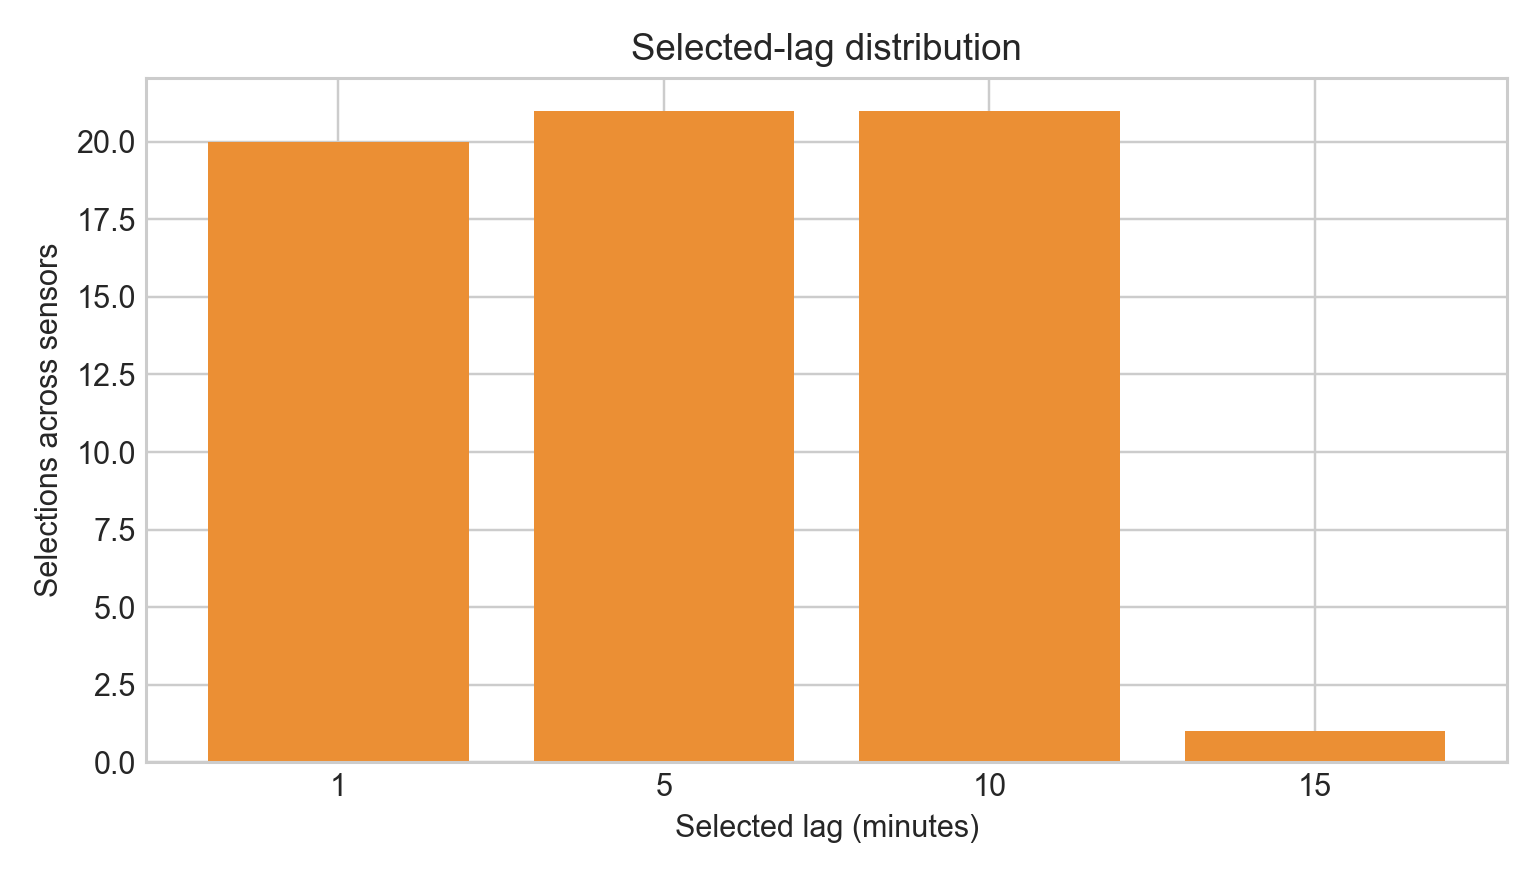
\includegraphics[width=.72\textwidth]{feature_preparation_artifacts/figures/selected_lag_distribution.png}\caption{Distribution of the 63 selected lags.}\end{figure}


\section{Compact temporal engineering}
\decision Each sensor receives a small, consistent temporal description instead of every statistic at every window.
\implementation The executed families are current value; three selected lags; 10- and 30-minute trailing means; 10-minute trailing standard deviation; five-minute difference; and 10-minute rolling slope. Windows are trailing and require complete history.
\actual The temporal candidate block contains 189 features before missingness indicators: 21 raw, 63 selected lags, 42 means, and 21 each for variability, difference, and trend.
\modelmeaning Raw values encode present state; lags encode delayed response; means encode recent level; standard deviation encodes instability; differences encode movement; slopes encode direction.
\limitation The same summary windows are used across sensors after lag selection. Later ablation should test whether every retained family earns its complexity.


\begin{table}[H]
\centering
\small
\begin{tabular}{p{0.25\textwidth}r p{0.53\textwidth}}
\toprule
Family & Candidates & Modeling hypothesis \\
\midrule
\nolinkurl{difference} & 21 & recent movement \\
\nolinkurl{raw} & 21 & current process state \\
\nolinkurl{rolling_mean} & 42 & recent operating level \\
\nolinkurl{selected_lag} & 63 & delayed process response \\
\nolinkurl{trend} & 21 & short-term direction \\
\nolinkurl{variability} & 21 & short-term instability \\
\bottomrule
\end{tabular}
\caption{Temporal-feature family counts from the executed notebook.}
\end{table}

\begin{figure}[H]\centering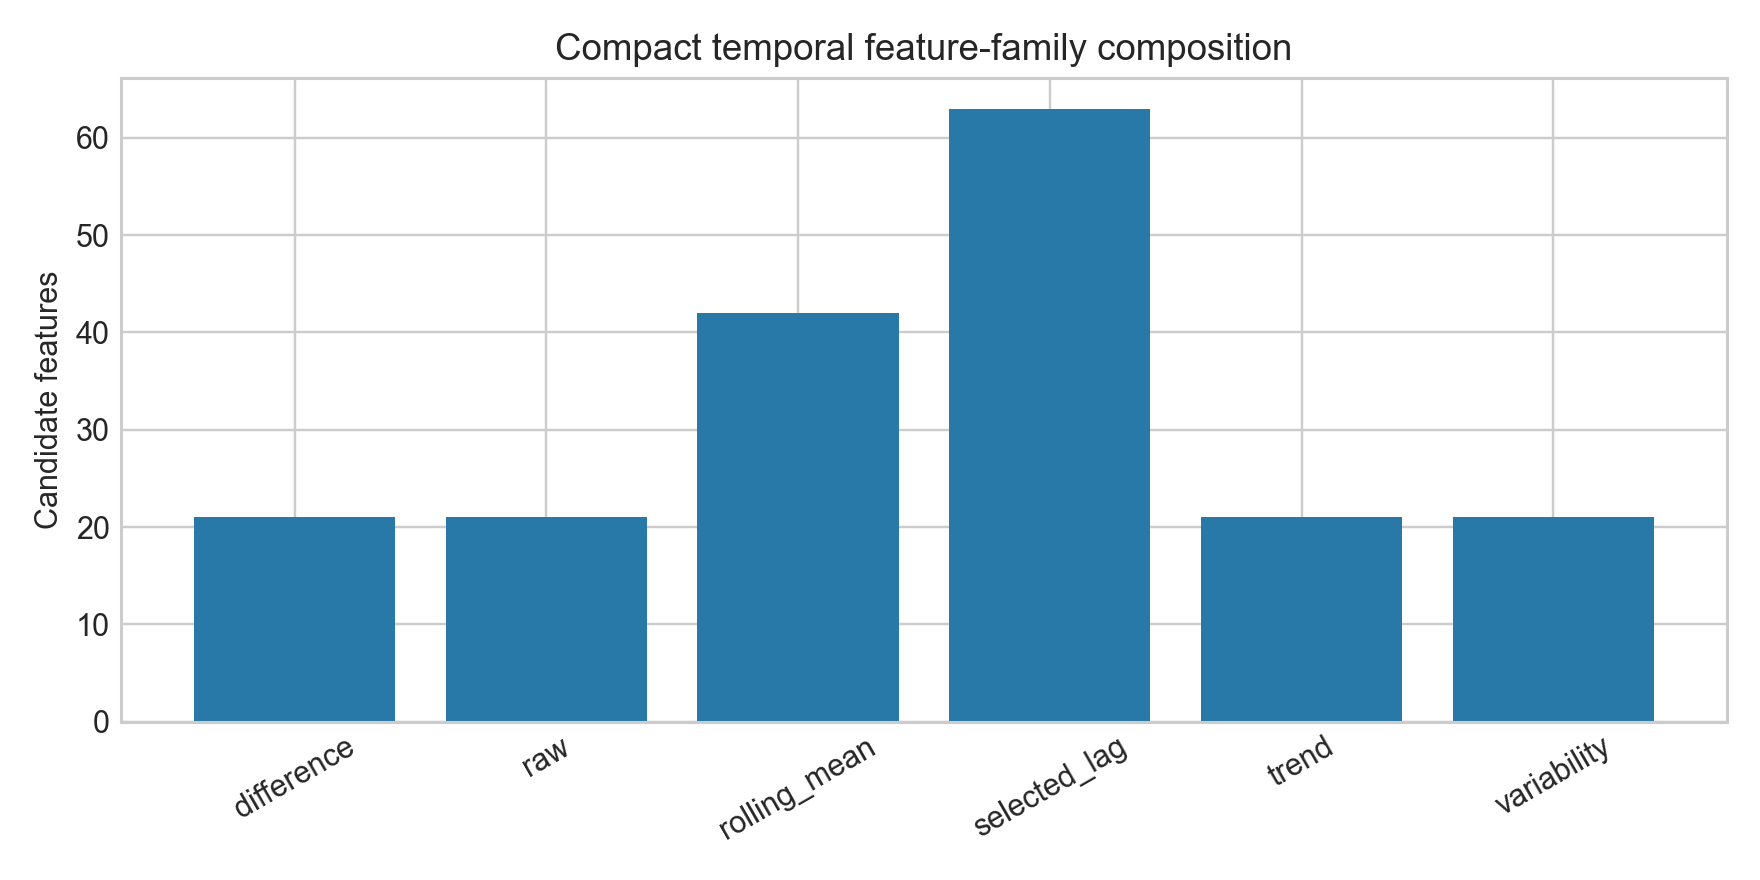
\includegraphics[width=.72\textwidth]{feature_preparation_artifacts/figures/feature_family_composition.png}\caption{Compact temporal candidate composition.}\end{figure}


\section{Process-aware features and validation metadata}
\decision Physical relationships are explicit experimental features, never undocumented interactions.
\implementation Each derived feature stores its exact formula, source tags, expected interpretation, assumptions, and validation status. Five coefficient-of-variation indicators use a 10-minute standard deviation divided by the magnitude of the 10-minute mean.
\actual Sixteen process-aware features were created: eleven balances, totals, ratios, gradients, or operating proxies, plus five flow-stability indicators. The total slurry volumetric flow is a confirmed m$^3$/h aggregation; the total acid aggregation is confirmed while its unit remains pending; eleven features remain provisional and three require mass-stream, unit, or engineering validation.
\modelmeaning These features test whether engineering relationships generalize better and explain more clearly than sensor-by-sensor statistics.
\limitation None is a verified physical quantity solely because it appears in this registry. In particular, pressure times temperature is a steam-condition model proxy, not energy or enthalpy.


\begin{landscape}\tiny\begin{longtable}{p{0.17\linewidth}p{0.19\linewidth}p{0.20\linewidth}p{0.14\linewidth}p{0.18\linewidth}p{0.10\linewidth}}\caption{Complete process-aware feature registry.}\\\toprule Feature & Formula & Inputs & Expected interpretation & Assumptions & Status \\\midrule\endfirsthead\toprule Feature & Formula & Inputs & Interpretation & Assumptions & Status \\\midrule\endhead
\nolinkurl{TOTAL_ACID_FLOW} & \nolinkurl{acid_1 + acid_2} & \nolinkurl{FLOW_RATE_PHOSPHORIC_ACID_1; FLOW_RATE_PHOSPHORIC_ACID_2} & Combined phosphoric-acid feed across both lines. & The two acid lines are confirmed additive; their engineering unit still requires confirmation. & \nolinkurl{aggregation_confirmed_units_pending} \\
\nolinkurl{ACID_FLOW_IMBALANCE} & \nolinkurl{|acid_1 - acid_2|} & \nolinkurl{FLOW_RATE_PHOSPHORIC_ACID_1; FLOW_RATE_PHOSPHORIC_ACID_2} & Magnitude of line imbalance. & The lines are comparable and imbalance is operationally meaningful. & \nolinkurl{provisional} \\
\nolinkurl{ACID_TO_PHOSPHATE_RATIO} & \nolinkurl{(acid_1 + acid_2) / (ground_phosphate + epsilon)} & \nolinkurl{FLOW_RATE_PHOSPHORIC_ACID_1; FLOW_RATE_PHOSPHORIC_ACID_2; FLOW_RATE_GROUND_PHOSPHATE} & Feed-ratio proxy related to acidulation conditions. & Flow units/bases are compatible; not a stoichiometric ratio without composition data. & \nolinkurl{provisional} \\
\nolinkurl{TOTAL_SLURRY_M3_FLOW} & \nolinkurl{slurry_m3_1 + slurry_m3_2} & \nolinkurl{FLOW_RATE_SLURRY_M3_HR; FLOW_RATE_SLURRY_M3_HR_2} & Confirmed total slurry volumetric flow in m3/h. & Both tags are confirmed additive components with the same m3/h unit. & \nolinkurl{confirmed_m3_per_h_aggregation} \\
\nolinkurl{SLURRY_DENSITY_PROXY} & \nolinkurl{slurry_t_per_h / (slurry_m3_1 + slurry_m3_2 + epsilon)} & \nolinkurl{FLOW_RATE_SLURRY_T_PER_HR; FLOW_RATE_SLURRY_M3_HR; FLOW_RATE_SLURRY_M3_HR_2} & Apparent slurry mass-per-volume proxy using total volumetric flow. & The two volumetric tags are confirmed additive in m3/h; confirm that the t/h tag represents the same combined stream. & \nolinkurl{requires_mass_stream_validation} \\
\nolinkurl{ATTACK_PASSAGE_TEMP_GRADIENT} & \nolinkurl{T_attack - T_passage} & \nolinkurl{TEMPERATURE_CUVE_ATTAQUE; TEMPERATURE_CUVE_DE_PASSAGE} & Thermal change between reaction vessels. & Sensors are comparable and process direction is attack to passage. & \nolinkurl{provisional} \\
\nolinkurl{HOT_AIR_DRYER_OUTLET_GRADIENT} & \nolinkurl{T_hot_air - T_dryer_outlet_gas} & \nolinkurl{TEMPERATURE_AIR_CHAUD; TEMPERATURE_GAZ_SORTIE_SECHEUR} & Dryer thermal-driving-force proxy. & Temperatures correspond to the same dryer train. & \nolinkurl{provisional} \\
\nolinkurl{STEAM_SLURRY_TEMP_GRADIENT} & \nolinkurl{T_steam - T_slurry} & \nolinkurl{TEMPERATURE_VAPEUR; TEMPERATURE_SLURRY_PULVERISATEUR} & Available temperature-gap proxy. & Steam/slurry tags belong to the relevant heat-transfer path. & \nolinkurl{provisional} \\
\nolinkurl{STEAM_ENERGY_PROXY} & \nolinkurl{steam_pressure * steam_temperature} & \nolinkurl{PRESSURE_VAPEUR; TEMPERATURE_VAPEUR} & Steam-condition proxy, not energy or enthalpy. & Tags refer to the same steam supply; units remain unconverted. & \nolinkurl{provisional} \\
\nolinkurl{DRYING_INTENSITY_PROXY} & \nolinkurl{fuel_flow * (T_hot_air - T_outlet) / (|dryer_depression| + epsilon)} & \nolinkurl{FLOW_RATE_FIOUL; TEMPERATURE_AIR_CHAUD; TEMPERATURE_GAZ_SORTIE_SECHEUR; DEPRESSURE_SECHEUR} & Composite burner/load/draft indicator. & Signs and units are not thermodynamically normalized; engineering review required. & \nolinkurl{requires_engineering_validation} \\
\nolinkurl{RECYCLE_TO_PRODUCTION_RATIO} & \nolinkurl{recycle / (production + epsilon)} & \nolinkurl{RECYCLAGE; PRODUCTION_TSP_BALANCE} & Recycle-intensity proxy. & Recycle and production tags use compatible mass/time bases. & \nolinkurl{requires_unit_validation} \\
\nolinkurl{FLOW_RATE_PHOSPHORIC_ACID_1_CV_10} & \nolinkurl{rolling_std_10(FLOW_RATE_PHOSPHORIC_ACID_1) / (|rolling_mean_10(FLOW_RATE_PHOSPHORIC_ACID_1)| + epsilon)} & \nolinkurl{FLOW_RATE_PHOSPHORIC_ACID_1} & Scale-normalized ten-minute flow instability. & Mean magnitude away from zero; extreme proxy values are clipped below. & \nolinkurl{provisional} \\
\nolinkurl{FLOW_RATE_PHOSPHORIC_ACID_2_CV_10} & \nolinkurl{rolling_std_10(FLOW_RATE_PHOSPHORIC_ACID_2) / (|rolling_mean_10(FLOW_RATE_PHOSPHORIC_ACID_2)| + epsilon)} & \nolinkurl{FLOW_RATE_PHOSPHORIC_ACID_2} & Scale-normalized ten-minute flow instability. & Mean magnitude away from zero; extreme proxy values are clipped below. & \nolinkurl{provisional} \\
\nolinkurl{FLOW_RATE_GROUND_PHOSPHATE_CV_10} & \nolinkurl{rolling_std_10(FLOW_RATE_GROUND_PHOSPHATE) / (|rolling_mean_10(FLOW_RATE_GROUND_PHOSPHATE)| + epsilon)} & \nolinkurl{FLOW_RATE_GROUND_PHOSPHATE} & Scale-normalized ten-minute flow instability. & Mean magnitude away from zero; extreme proxy values are clipped below. & \nolinkurl{provisional} \\
\nolinkurl{FLOW_RATE_FIOUL_CV_10} & \nolinkurl{rolling_std_10(FLOW_RATE_FIOUL) / (|rolling_mean_10(FLOW_RATE_FIOUL)| + epsilon)} & \nolinkurl{FLOW_RATE_FIOUL} & Scale-normalized ten-minute flow instability. & Mean magnitude away from zero; extreme proxy values are clipped below. & \nolinkurl{provisional} \\
\nolinkurl{FLOW_RATE_VAPEUR_CV_10} & \nolinkurl{rolling_std_10(FLOW_RATE_VAPEUR) / (|rolling_mean_10(FLOW_RATE_VAPEUR)| + epsilon)} & \nolinkurl{FLOW_RATE_VAPEUR} & Scale-normalized ten-minute flow instability. & Mean magnitude away from zero; extreme proxy values are clipped below. & \nolinkurl{provisional} \\\bottomrule\end{longtable}\end{landscape}

\begin{figure}[H]\centering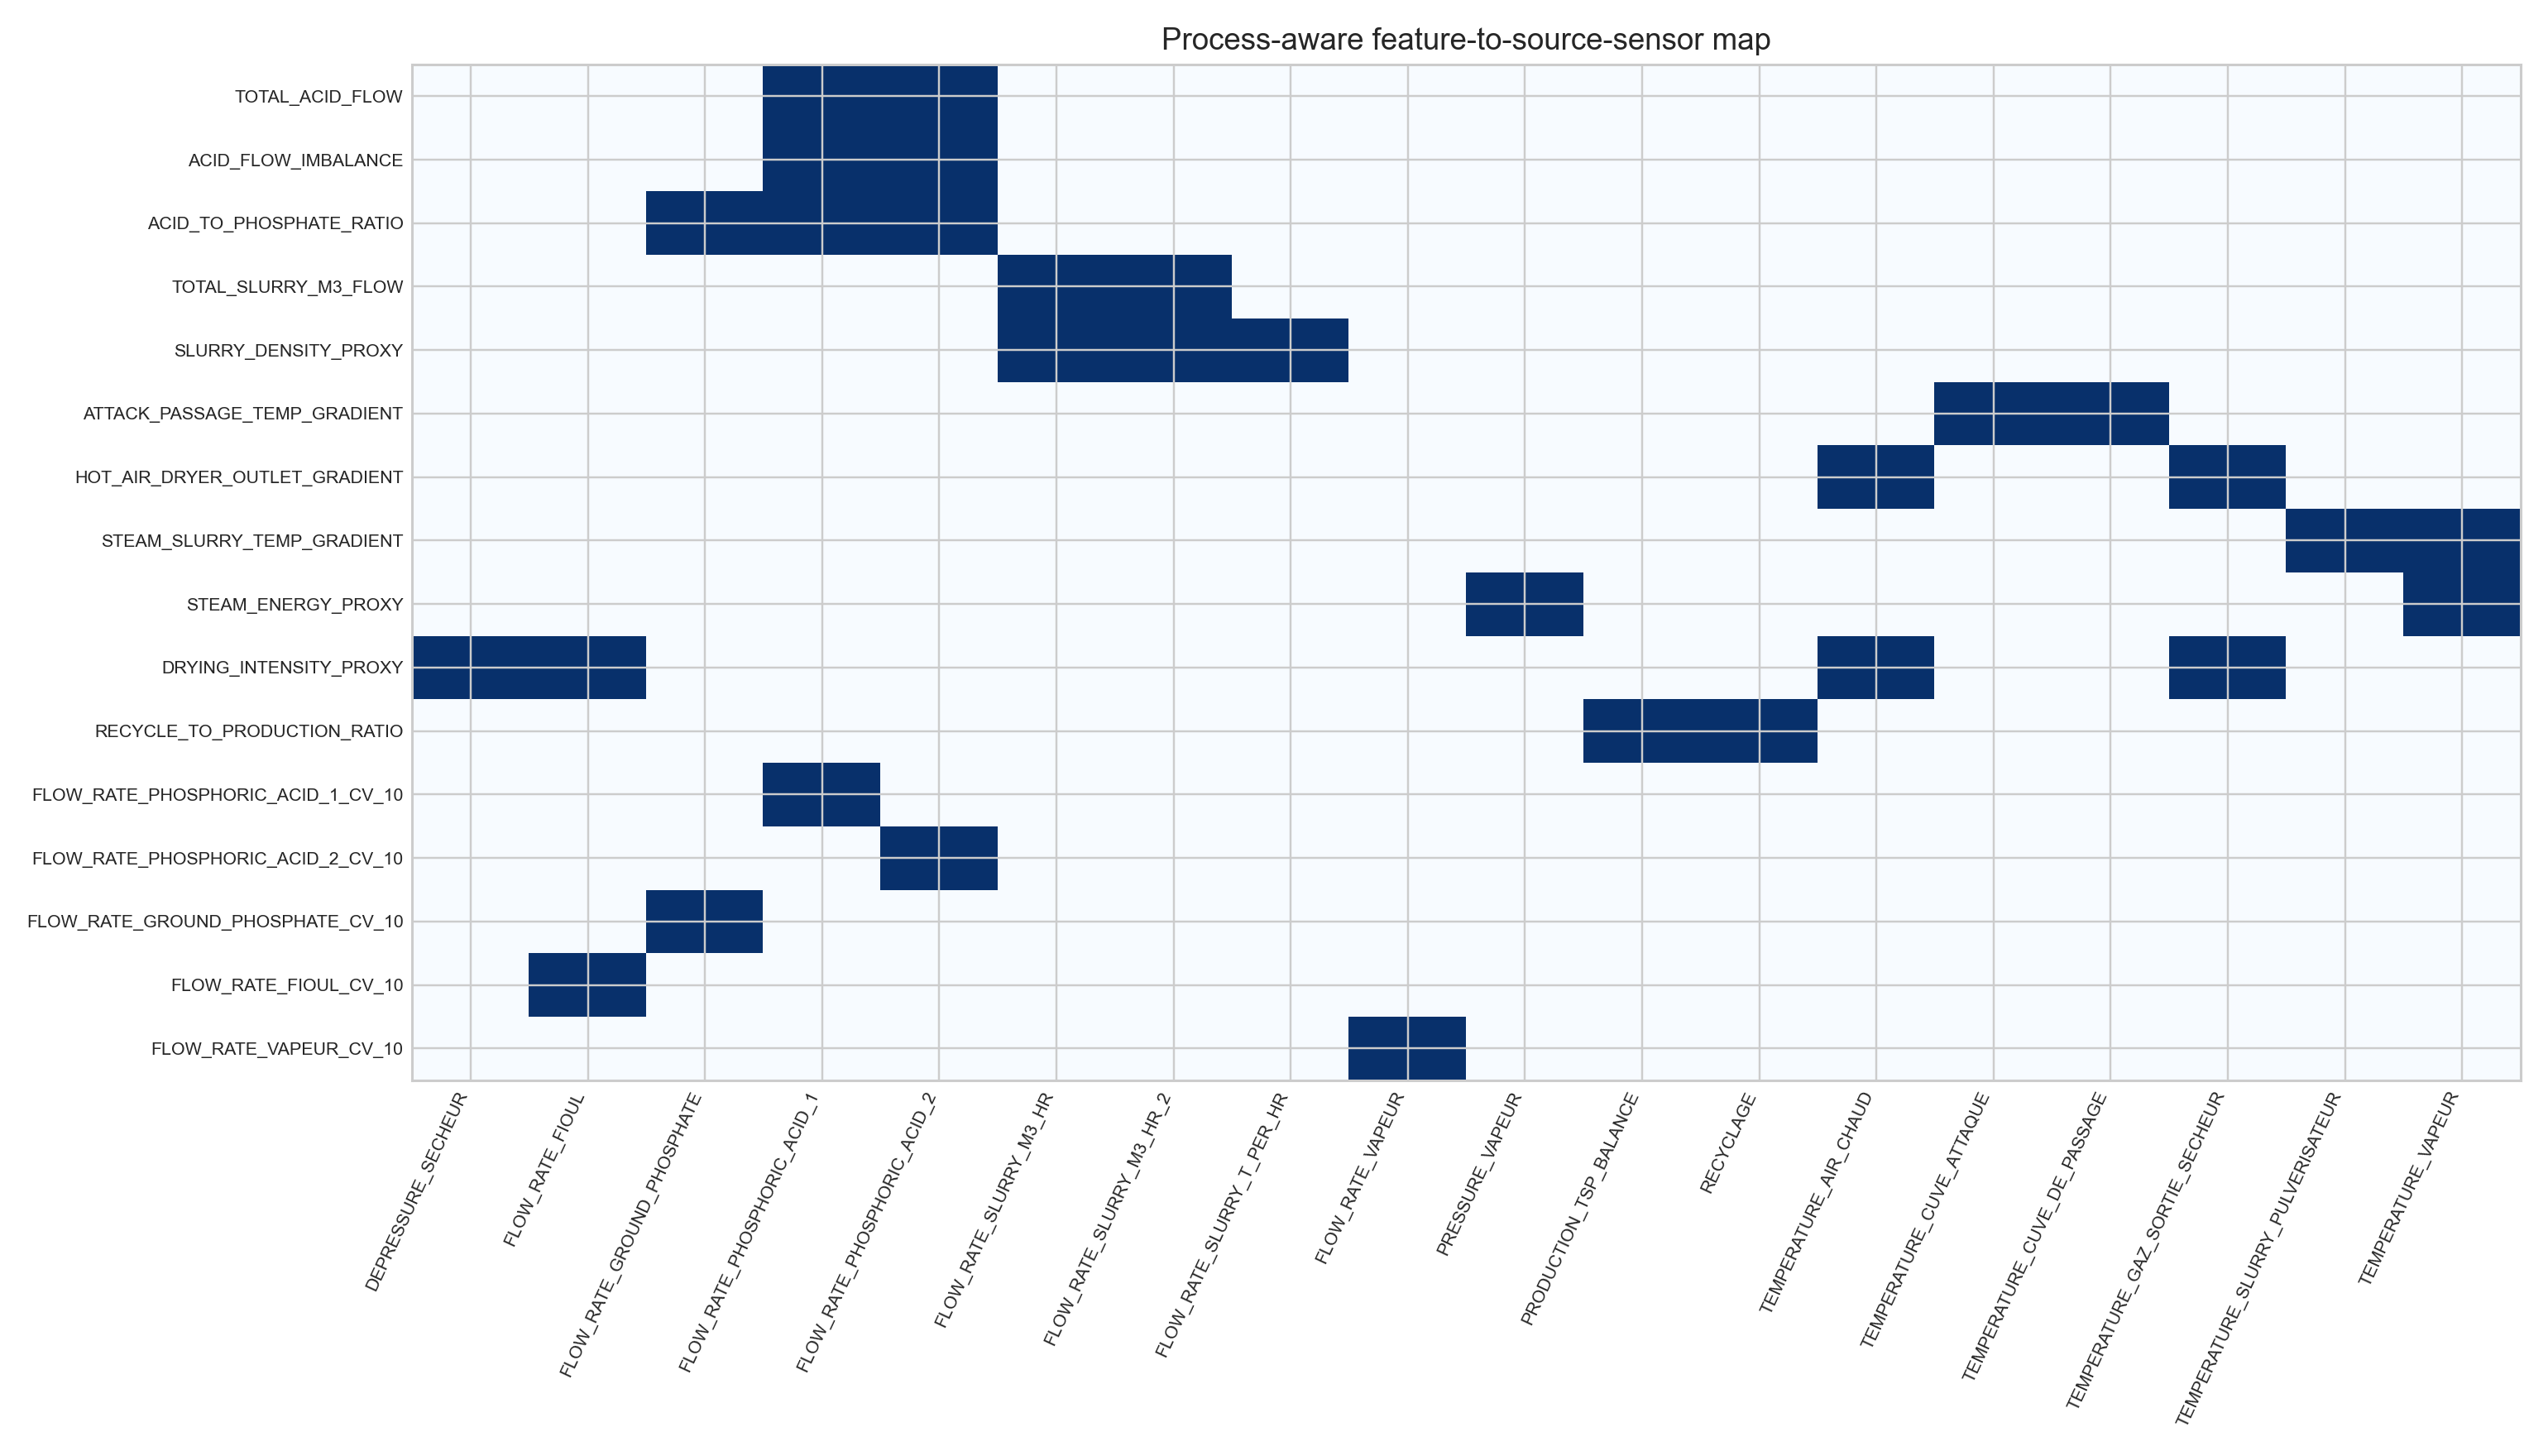
\includegraphics[width=.98\textwidth]{feature_preparation_artifacts/figures/process_feature_map.png}\caption{Process-aware features linked to their source sensors.}\end{figure}


\section{Guarded ratios, clipping, and numerical stability}
\decision Unbounded percentage changes are not generated because several sensors approach or cross zero.
\implementation The configured epsilon is $10^{-6}$. Guarded ratios are missing when $|d|\leq\epsilon$; otherwise the signed denominator receives a signed epsilon adjustment. Infinite values are replaced by missing values. Each process feature is clipped to its own 0.1st and 99.9th percentile bounds learned from the raw training period only, then applied unchanged to later periods.
\actual Sixteen feature-specific clipping pairs are exported in \texttt{process\_clipping\_bounds.csv}. The readiness audit confirms that these bounds use training data only.
\modelmeaning The controls limit near-zero explosions and extreme leverage without using validation/test distributions.
\limitation Quantile clipping is statistical protection, not a substitute for engineering plausibility limits. Negative source values and very large drying-proxy bounds indicate that sensor-quality and shutdown regimes need explicit review.

\section{Structural warm-up versus genuine missingness}
\decision Structurally unavailable history is removed, not median-imputed.
\implementation The maximum accepted lookback is 30 minutes (the largest selected lag is 15 minutes, but the medium rolling mean requires 30). Rows 0--29 are dropped before splitting. After this boundary, genuine gaps in all 21 sensor tags receive binary indicators in Sets B--D and median imputation fitted on training only. Set A remains strictly raw and contains no indicators.
\actual Exactly 30 rows were removed. The usable feature timeline begins at 2026-01-01 00:30 UTC. Twenty-one genuine-missingness indicators are available in Sets B, C, and D.
\modelmeaning Structural absence and sensor failure now have different treatments and interpretations.
\limitation A binary indicator identifies missingness but does not distinguish maintenance, communications failure, or process shutdown.


\begin{table}[H]
\centering
\small
\begin{tabular}{p{0.30\textwidth}r p{0.55\textwidth}}
\toprule
Policy & Rows & Reason \\
\midrule
\nolinkurl{drop_structural_warmup} & 30 & History does not exist for accepted lag/rolling features. \\
\nolinkurl{preserve_genuine_sensor_missingness} & 0 & Post-warm-up gaps receive indicators and train-fitted median imputation. \\
\bottomrule
\end{tabular}
\caption{Warm-up and genuine-missingness policy.}
\end{table}


\section{Four feature-set hypotheses}
\decision Four named input configurations replace one universal matrix.
\implementation Every configuration is independently filtered and preprocessed for every horizon, producing 16 experimental keys.
\actual Candidate widths are 21 (A), 210 (B), 58 (C), and 226 (D). Set A has no missing indicators; Sets B--D each include 21.
\modelmeaning Direct ablation can quantify predictive gain against complexity and physical interpretability.
\limitation Set C includes raw measurements as specified; it tests incremental process relationships rather than process features in isolation.


\begin{table}[H]
\centering
\footnotesize
\begin{tabular}{p{0.12\textwidth}p{0.38\textwidth}p{0.42\textwidth}}
\toprule
Set & Contents & Hypothesis \\
\midrule
\nolinkurl{A_raw} & Current sensor measurements only & The current process state alone contains sufficient predictive information. \\
\nolinkurl{B_temporal} & Raw plus selected lags, rolling levels, variability, difference, slope, and genuine missingness indicators & Selected process histories and recent dynamics improve forecasting. \\
\nolinkurl{C_process} & Raw plus balances, ratios, gradients, stability proxies, and genuine missingness indicators & Physically interpretable relationships improve prediction and generalization. \\
\nolinkurl{D_full} & Accepted temporal and process-aware features plus genuine missingness indicators & Temporal and process-relationship evidence are complementary. \\
\bottomrule
\end{tabular}
\caption{Feature-set definitions and hypotheses.}
\end{table}

\begin{figure}[H]\centering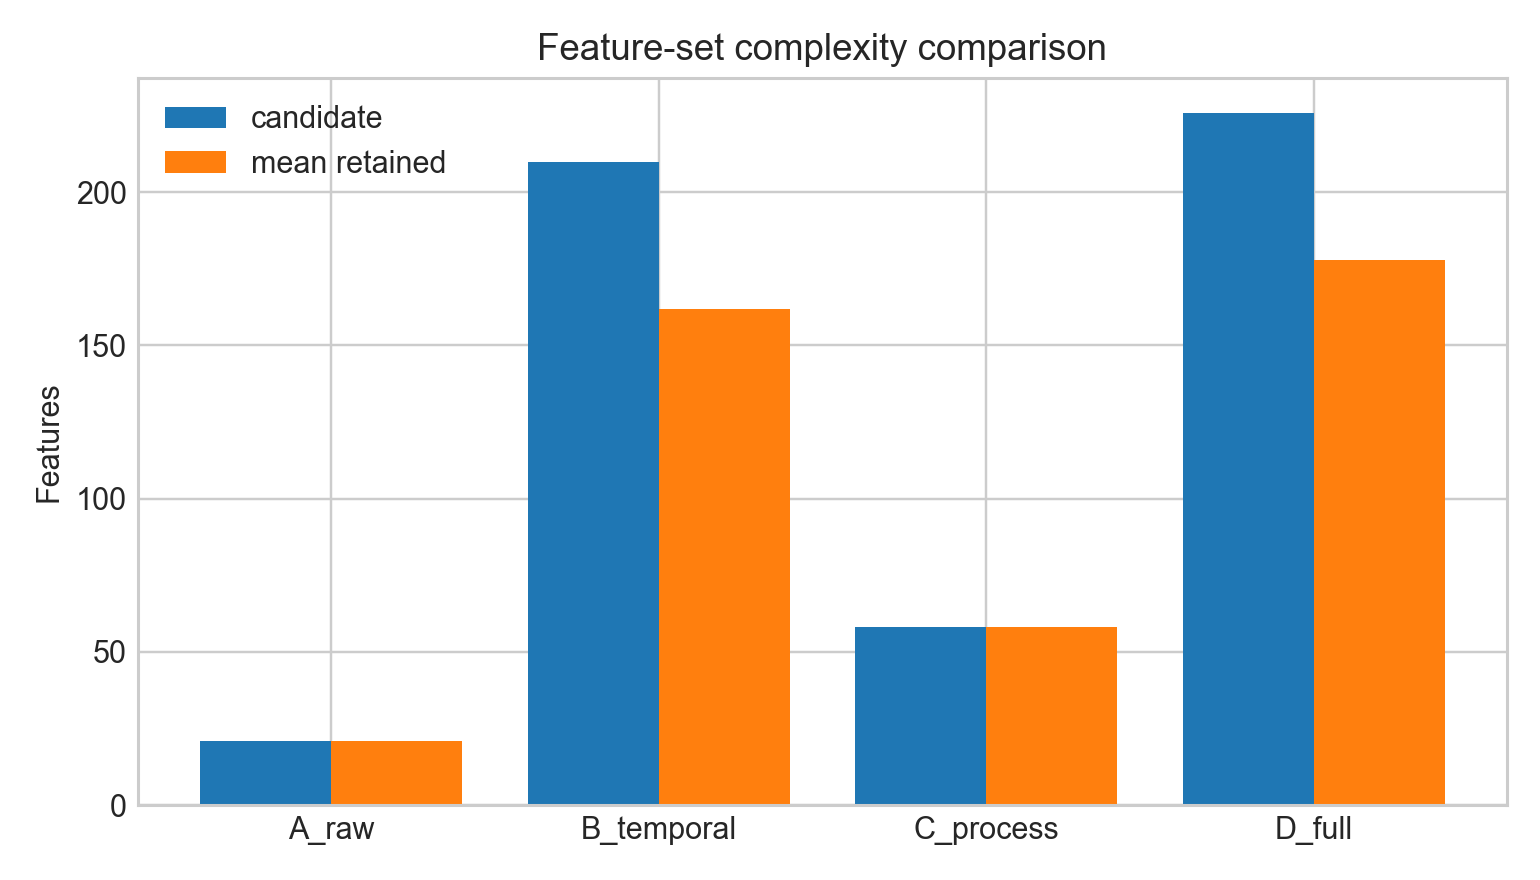
\includegraphics[width=.72\textwidth]{feature_preparation_artifacts/figures/feature_set_comparison.png}\caption{Candidate and mean retained feature counts by set.}\end{figure}


\section{Chronological splitting by horizon}
\decision All configurations use a 70/15/15 chronological policy without shuffling.
\implementation Target-missing rows are removed separately by horizon before integer split boundaries are calculated.
\actual Split endpoints differ by minutes as the horizon increases. There is no overlap: training precedes validation, which precedes test.
\modelmeaning Evaluation mimics forward deployment and prevents adjacent future observations from leaking backward through random allocation.
\limitation One holdout month and highly dependent one-minute samples do not quantify seasonal uncertainty; rolling-origin validation should follow.


\begin{table}[H]
\centering
\footnotesize
\begin{tabular}{rrr p{0.27\textwidth}p{0.27\textwidth}}
\toprule
Horizon & Split & Rows & Start (UTC) & End (UTC) \\
\midrule
1 & train & 31,011 & 2026-01-01 00:30:00+00:00 & 2026-01-22 17:17:00+00:00 \\
1 & validation & 6,645 & 2026-01-22 17:18:00+00:00 & 2026-01-27 08:58:00+00:00 \\
1 & test & 6,646 & 2026-01-27 08:59:00+00:00 & 2026-01-31 23:58:00+00:00 \\
5 & train & 31,008 & 2026-01-01 00:30:00+00:00 & 2026-01-22 17:14:00+00:00 \\
5 & validation & 6,645 & 2026-01-22 17:15:00+00:00 & 2026-01-27 08:55:00+00:00 \\
5 & test & 6,645 & 2026-01-27 08:56:00+00:00 & 2026-01-31 23:54:00+00:00 \\
10 & train & 31,005 & 2026-01-01 00:30:00+00:00 & 2026-01-22 17:11:00+00:00 \\
10 & validation & 6,644 & 2026-01-22 17:12:00+00:00 & 2026-01-27 08:51:00+00:00 \\
10 & test & 6,644 & 2026-01-27 08:52:00+00:00 & 2026-01-31 23:49:00+00:00 \\
15 & train & 31,001 & 2026-01-01 00:30:00+00:00 & 2026-01-22 17:07:00+00:00 \\
15 & validation & 6,643 & 2026-01-22 17:08:00+00:00 & 2026-01-27 08:46:00+00:00 \\
15 & test & 6,644 & 2026-01-27 08:47:00+00:00 & 2026-01-31 23:44:00+00:00 \\
\bottomrule
\end{tabular}
\caption{Exact chronological boundaries by target horizon.}
\end{table}

\begin{figure}[H]\centering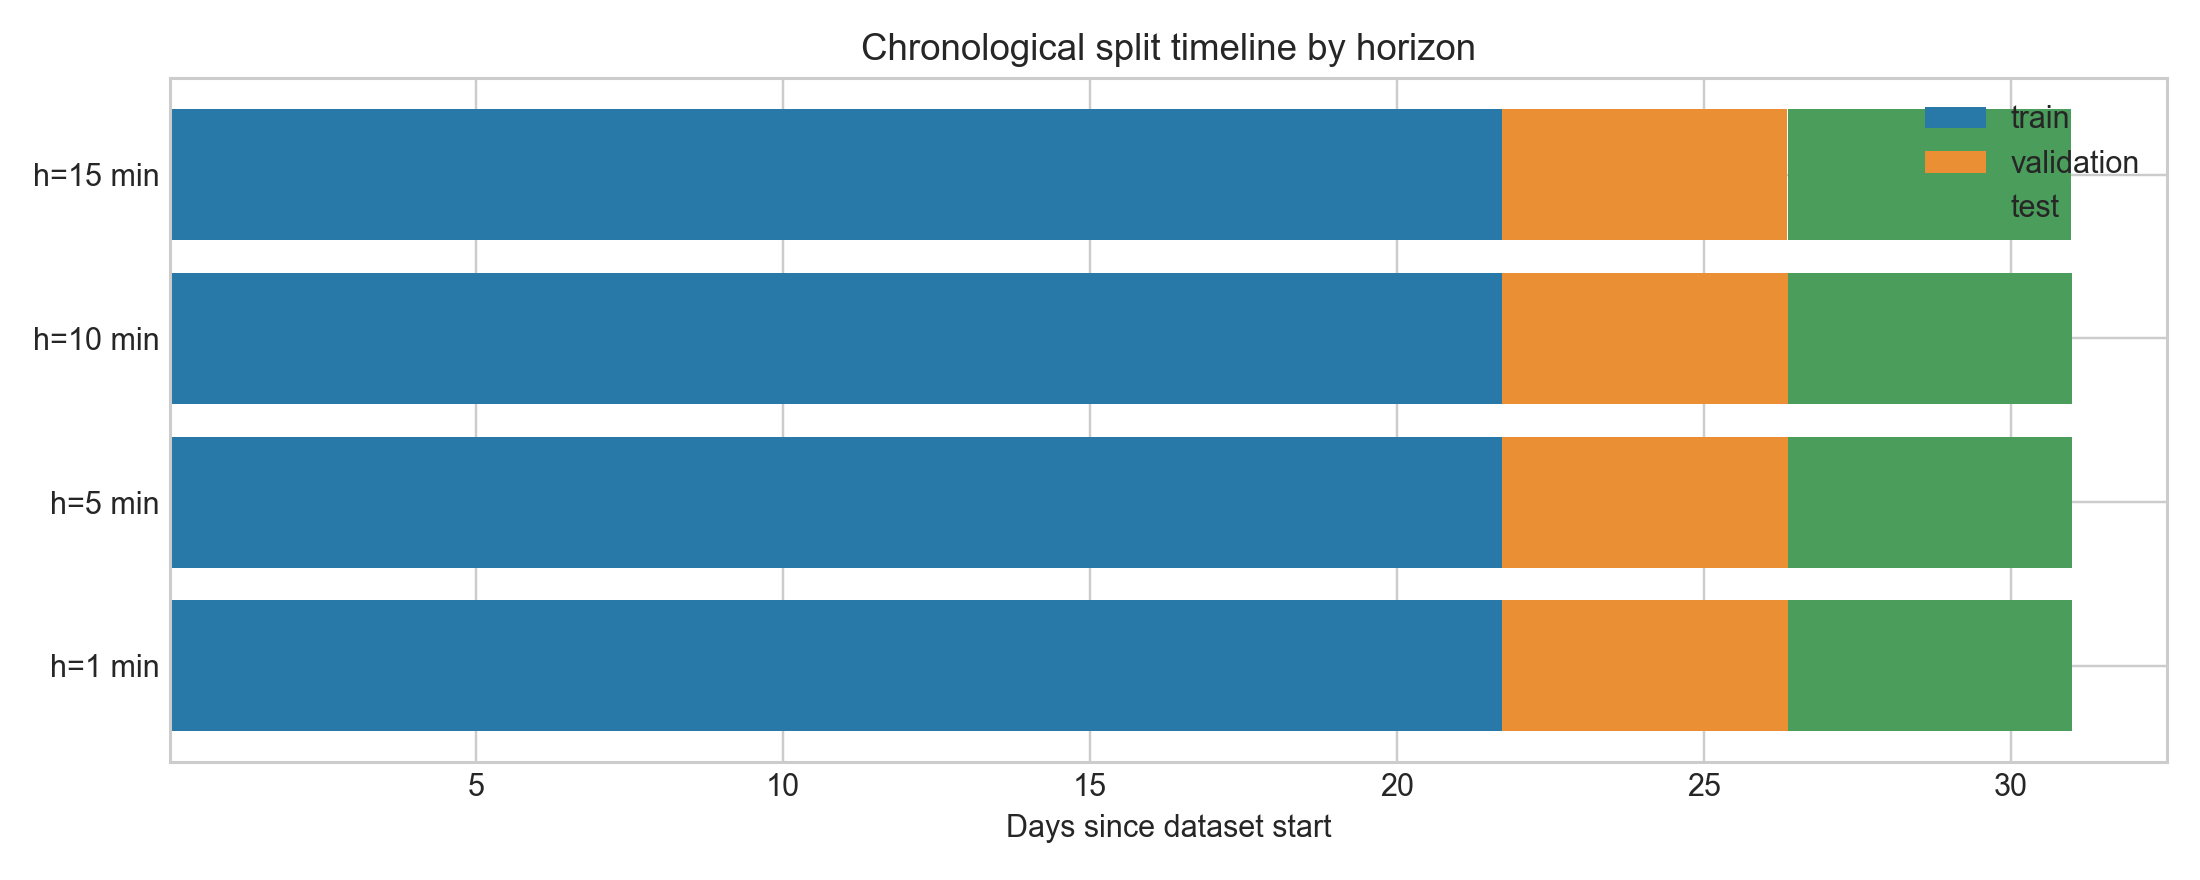
\includegraphics[width=.88\textwidth]{feature_preparation_artifacts/figures/split_timeline.png}\caption{Chronological split timeline by horizon.}\end{figure}


\section{Grouped, interpretability-aware correlation filtering}
\decision Correlation filtering is limited to features from the same original sensor; process-aware features and missingness indicators are protected.
\implementation The filter is fitted separately on the training matrix for each horizon and set at $|r|>0.98$. Priority is: (1) raw value, (2) selected lag, (3) rolling mean, (4) difference, (5) slope, and (6) variability. Each removal records both features, absolute correlation, source sensor, and reason.
\actual Sets A and C lose no features. Sets B and D each remove 48 and retain 162 and 178 respectively at every horizon.
\modelmeaning High correlation within a source family can be reduced while semantically distinct balances, ratios, gradients, and stability proxies remain available for ablation.
\limitation During transitions, a raw value and lag may behave differently despite high full-period correlation. The log should be revisited for transition-focused models.


\begin{table}[H]
\centering
\small
\begin{tabular}{rrrrr}
\toprule
Horizon & Set & Candidate & Retained & Removed \\
\midrule
1 & \nolinkurl{A_raw} & 21 & 21 & 0 \\
1 & \nolinkurl{B_temporal} & 210 & 162 & 48 \\
1 & \nolinkurl{C_process} & 58 & 58 & 0 \\
1 & \nolinkurl{D_full} & 226 & 178 & 48 \\
5 & \nolinkurl{A_raw} & 21 & 21 & 0 \\
5 & \nolinkurl{B_temporal} & 210 & 162 & 48 \\
5 & \nolinkurl{C_process} & 58 & 58 & 0 \\
5 & \nolinkurl{D_full} & 226 & 178 & 48 \\
10 & \nolinkurl{A_raw} & 21 & 21 & 0 \\
10 & \nolinkurl{B_temporal} & 210 & 162 & 48 \\
10 & \nolinkurl{C_process} & 58 & 58 & 0 \\
10 & \nolinkurl{D_full} & 226 & 178 & 48 \\
15 & \nolinkurl{A_raw} & 21 & 21 & 0 \\
15 & \nolinkurl{B_temporal} & 210 & 162 & 48 \\
15 & \nolinkurl{C_process} & 58 & 58 & 0 \\
15 & \nolinkurl{D_full} & 226 & 178 & 48 \\
\bottomrule
\end{tabular}
\caption{Grouped filtering results by horizon and feature set.}
\end{table}

\begin{landscape}\scriptsize\begin{longtable}{p{0.25\linewidth}p{0.25\linewidth}r p{0.23\linewidth}p{0.20\linewidth}}\caption{Representative correlation-removal decisions (one-minute temporal set).}\\\toprule Removed & Retained & $|r|$ & Source sensor & Reason \\\midrule
\nolinkurl{PRODUCTION_TSP_BALANCE_lag_1} & \nolinkurl{PRODUCTION_TSP_BALANCE} & 0.9924 & \nolinkurl{PRODUCTION_TSP_BALANCE} & Same family; retained more interpretable representative \\
\nolinkurl{PRODUCTION_TSP_BALANCE_lag_10} & \nolinkurl{PRODUCTION_TSP_BALANCE} & 0.9805 & \nolinkurl{PRODUCTION_TSP_BALANCE} & Same family; retained more interpretable representative \\
\nolinkurl{PRODUCTION_TSP_BALANCE_lag_5} & \nolinkurl{PRODUCTION_TSP_BALANCE} & 0.9881 & \nolinkurl{PRODUCTION_TSP_BALANCE} & Same family; retained more interpretable representative \\
\nolinkurl{PRODUCTION_TSP_BALANCE_roll_mean_10} & \nolinkurl{PRODUCTION_TSP_BALANCE} & 0.9815 & \nolinkurl{PRODUCTION_TSP_BALANCE} & Same family; retained more interpretable representative \\
\nolinkurl{FLOW_RATE_PHOSPHORIC_ACID_1_lag_1} & \nolinkurl{FLOW_RATE_PHOSPHORIC_ACID_1} & 0.9922 & \nolinkurl{FLOW_RATE_PHOSPHORIC_ACID_1} & Same family; retained more interpretable representative \\
\nolinkurl{FLOW_RATE_PHOSPHORIC_ACID_1_lag_5} & \nolinkurl{FLOW_RATE_PHOSPHORIC_ACID_1} & 0.9860 & \nolinkurl{FLOW_RATE_PHOSPHORIC_ACID_1} & Same family; retained more interpretable representative \\
\nolinkurl{FLOW_RATE_PHOSPHORIC_ACID_2_lag_1} & \nolinkurl{FLOW_RATE_PHOSPHORIC_ACID_2} & 0.9928 & \nolinkurl{FLOW_RATE_PHOSPHORIC_ACID_2} & Same family; retained more interpretable representative \\
\nolinkurl{FLOW_RATE_PHOSPHORIC_ACID_2_lag_5} & \nolinkurl{FLOW_RATE_PHOSPHORIC_ACID_2} & 0.9874 & \nolinkurl{FLOW_RATE_PHOSPHORIC_ACID_2} & Same family; retained more interpretable representative \\\bottomrule\end{longtable}\end{landscape}

\begin{figure}[H]\centering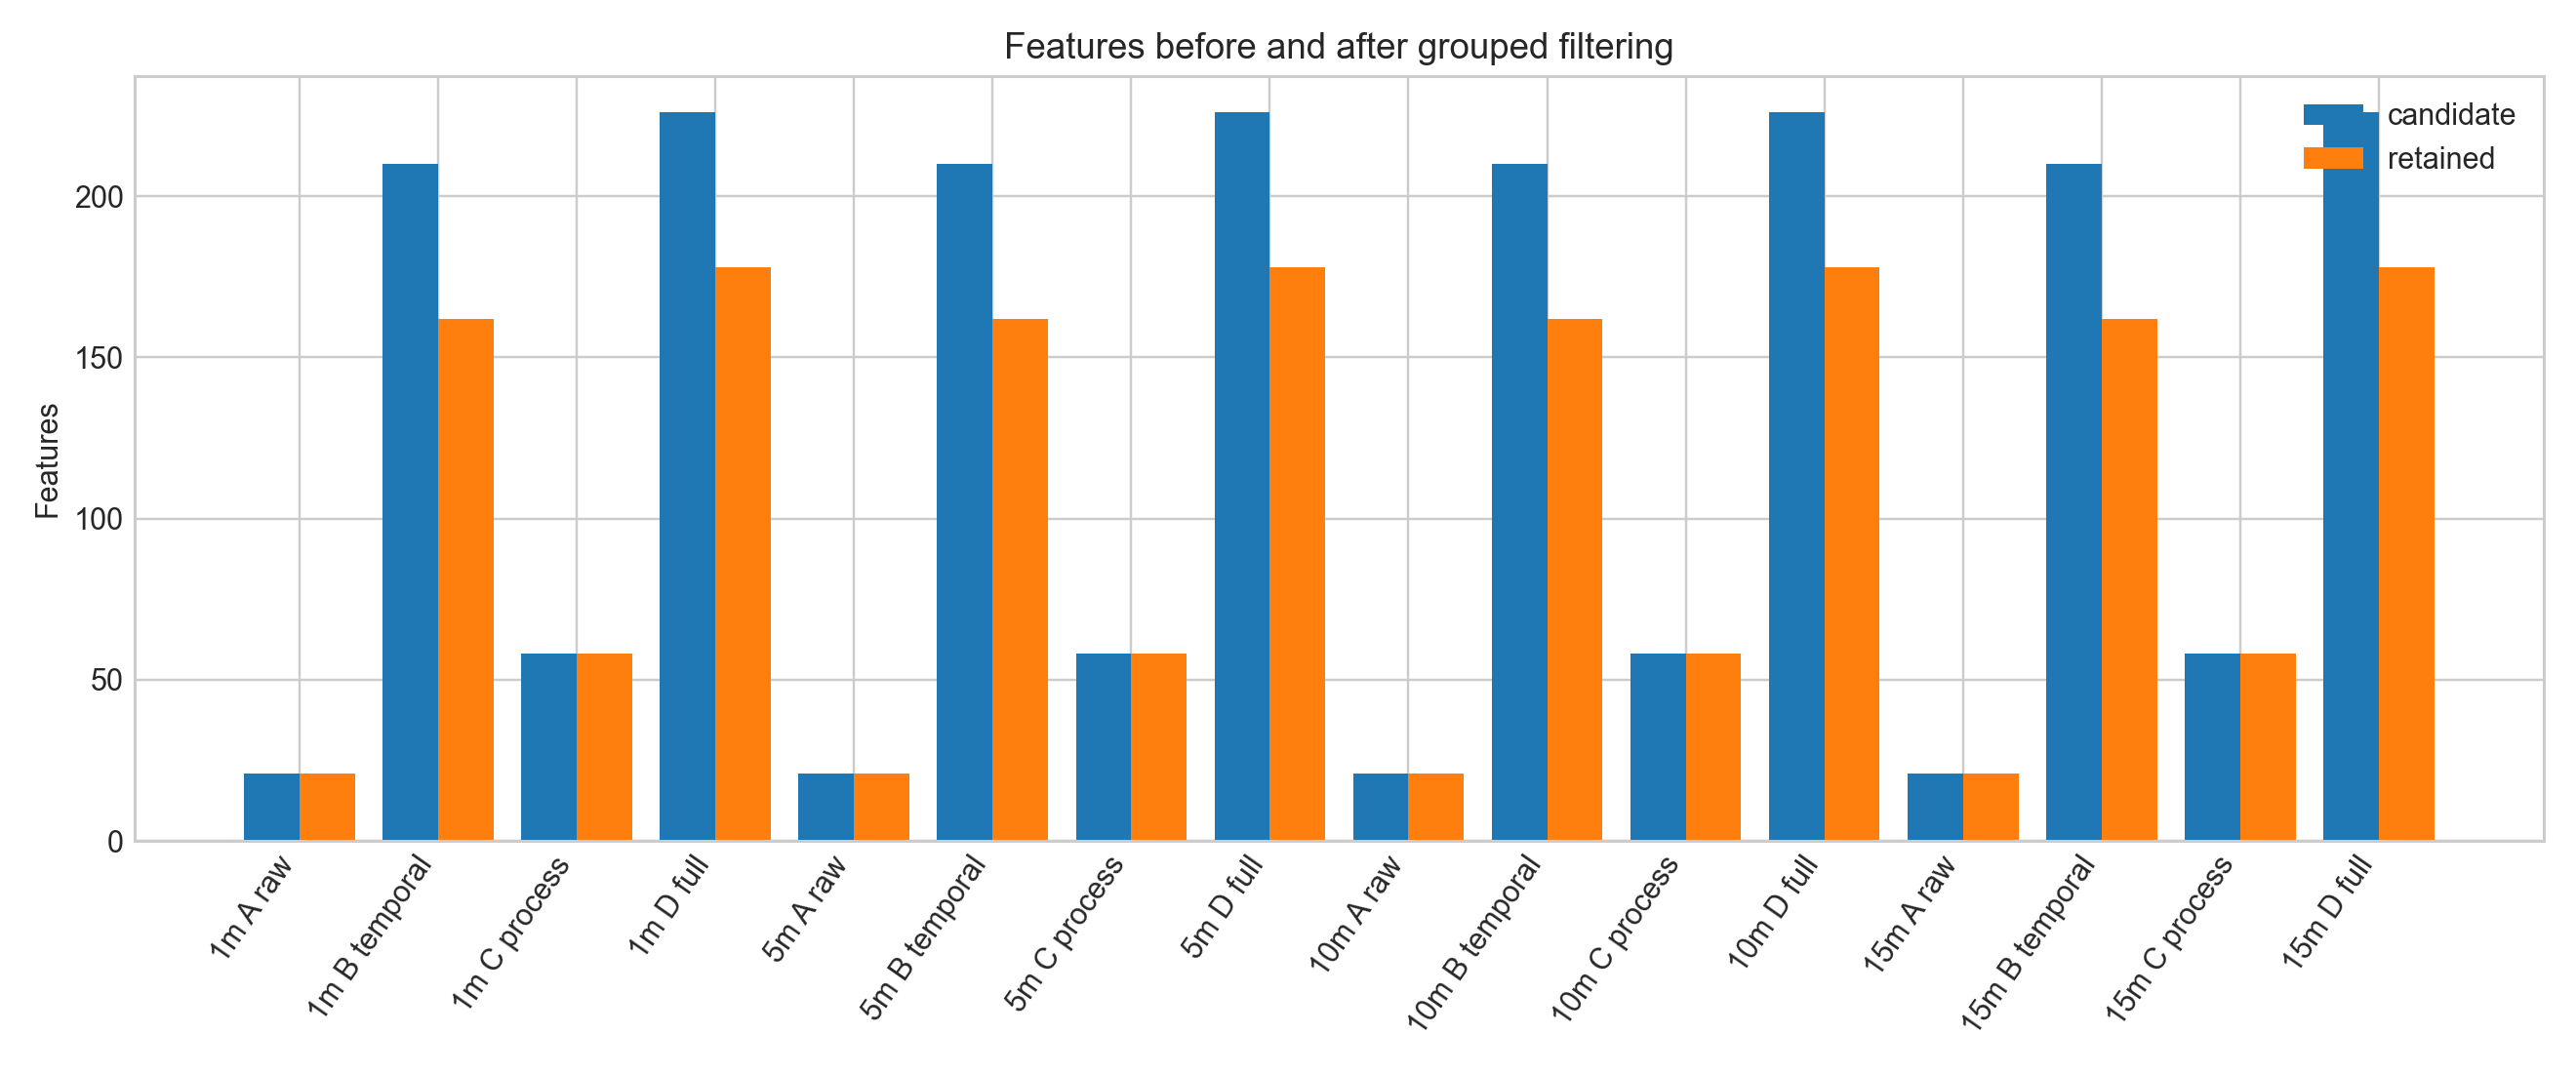
\includegraphics[width=.98\textwidth]{feature_preparation_artifacts/figures/feature_counts_before_after.png}\caption{Features before and after grouped filtering for all 16 configurations.}\end{figure}


\section{Final dimensions and preprocessing variants}
\decision Each horizon--set pair has four preprocessing variants.
\implementation Median imputers and any scaler are fitted on training only. Validation and test are transformed without refitting and retain identical ordered columns.
\actual The artifact dictionary contains 16 experiment keys and four variants per key: unscaled tree, robust, standard, and MinMax. No post-transform missing values remain.
\modelmeaning Algorithm comparisons can use appropriate scaling without changing data partitions or feature definitions.
\limitation MinMax values can leave the training range in future operation; this must be monitored rather than silently clipped.


\begin{landscape}\footnotesize\begin{longtable}{rrr r r rrr}\caption{Final matrix dimensions; cells show rows $\times$ columns.}\\\toprule Horizon & Set & Candidate & Retained & Indicators & Train & Validation & Test \\\midrule\endfirsthead\toprule Horizon & Set & Candidate & Retained & Indicators & Train & Validation & Test \\\midrule\endhead
1 & \nolinkurl{A_raw} & 21 & 21 & 0 & 31,011 x 21 & 6,645 x 21 & 6,646 x 21 \\
1 & \nolinkurl{B_temporal} & 210 & 162 & 21 & 31,011 x 162 & 6,645 x 162 & 6,646 x 162 \\
1 & \nolinkurl{C_process} & 58 & 58 & 21 & 31,011 x 58 & 6,645 x 58 & 6,646 x 58 \\
1 & \nolinkurl{D_full} & 226 & 178 & 21 & 31,011 x 178 & 6,645 x 178 & 6,646 x 178 \\
5 & \nolinkurl{A_raw} & 21 & 21 & 0 & 31,008 x 21 & 6,645 x 21 & 6,645 x 21 \\
5 & \nolinkurl{B_temporal} & 210 & 162 & 21 & 31,008 x 162 & 6,645 x 162 & 6,645 x 162 \\
5 & \nolinkurl{C_process} & 58 & 58 & 21 & 31,008 x 58 & 6,645 x 58 & 6,645 x 58 \\
5 & \nolinkurl{D_full} & 226 & 178 & 21 & 31,008 x 178 & 6,645 x 178 & 6,645 x 178 \\
10 & \nolinkurl{A_raw} & 21 & 21 & 0 & 31,005 x 21 & 6,644 x 21 & 6,644 x 21 \\
10 & \nolinkurl{B_temporal} & 210 & 162 & 21 & 31,005 x 162 & 6,644 x 162 & 6,644 x 162 \\
10 & \nolinkurl{C_process} & 58 & 58 & 21 & 31,005 x 58 & 6,644 x 58 & 6,644 x 58 \\
10 & \nolinkurl{D_full} & 226 & 178 & 21 & 31,005 x 178 & 6,644 x 178 & 6,644 x 178 \\
15 & \nolinkurl{A_raw} & 21 & 21 & 0 & 31,001 x 21 & 6,643 x 21 & 6,644 x 21 \\
15 & \nolinkurl{B_temporal} & 210 & 162 & 21 & 31,001 x 162 & 6,643 x 162 & 6,644 x 162 \\
15 & \nolinkurl{C_process} & 58 & 58 & 21 & 31,001 x 58 & 6,643 x 58 & 6,644 x 58 \\
15 & \nolinkurl{D_full} & 226 & 178 & 21 & 31,001 x 178 & 6,643 x 178 & 6,644 x 178 \\\bottomrule\end{longtable}\end{landscape}

\begin{table}[H]
\centering
\small
\begin{tabular}{p{0.13\textwidth}p{0.37\textwidth}p{0.42\textwidth}}
\toprule
Variant & Transformation & Intended model families \\
\midrule
\nolinkurl{tree} & training-median imputation; no scaling & tree ensembles and gradient boosting \\
\nolinkurl{robust} & training-median imputation; RobustScaler & outlier-aware linear and neural baselines \\
\nolinkurl{standard} & training-median imputation; StandardScaler & regularized linear models, PCA, diagnostics \\
\nolinkurl{minmax} & training-median imputation; MinMaxScaler & bounded-input neural baselines \\
\bottomrule
\end{tabular}
\caption{Preprocessing variants created for every horizon and feature set.}
\end{table}


\section{Readiness audit}
The notebook's final assertions verify execution integrity, time order, leakage boundaries, configuration completeness, fitted preprocessing, column alignment, missing-value removal, populated registries/logs, intervention safety, artifact exports, and the absence of model training. ``Current or past only'' is an implementation invariant: target shifts are confined to target creation; sensor lag operations use positive shifts and trailing windows.


\begin{table}[H]
\centering
\footnotesize
\begin{tabular}{p{0.78\textwidth}p{0.12\textwidth}}
\toprule
Validation check & Result \\
\midrule
\nolinkurl{chronological_order_preserved_for_every_horizon} & \textcolor{passgreen}{\textbf{PASS}} \\
\nolinkurl{four_future_targets_created} & \textcolor{passgreen}{\textbf{PASS}} \\
\nolinkurl{target_and_future_targets_absent_from_inputs} & \textcolor{passgreen}{\textbf{PASS}} \\
\nolinkurl{lag_transformations_match_positive_historical_shifts} & \textcolor{passgreen}{\textbf{PASS}} \\
\nolinkurl{all_four_feature_sets_prepared_for_every_horizon} & \textcolor{passgreen}{\textbf{PASS}} \\
\nolinkurl{preprocessor_imputation_statistics_match_training_data} & \textcolor{passgreen}{\textbf{PASS}} \\
\nolinkurl{train_validation_test_columns_aligned} & \textcolor{passgreen}{\textbf{PASS}} \\
\nolinkurl{all_prepared_matrices_have_no_missing_values} & \textcolor{passgreen}{\textbf{PASS}} \\
\nolinkurl{selection_cutoff_precedes_every_validation_period} & \textcolor{passgreen}{\textbf{PASS}} \\
\nolinkurl{process_clipping_bounds_use_selection_training_period_only} & \textcolor{passgreen}{\textbf{PASS}} \\
\nolinkurl{structural_warmup_removed_before_splitting} & \textcolor{passgreen}{\textbf{PASS}} \\
\nolinkurl{registries_and_filtering_log_populated} & \textcolor{passgreen}{\textbf{PASS}} \\
\nolinkurl{no_change_recommendations_authorized} & \textcolor{passgreen}{\textbf{PASS}} \\
\nolinkurl{no_predictive_model_trained_in_notebook} & \textcolor{passgreen}{\textbf{PASS}} \\
\nolinkurl{all_expected_exported_artifacts_exist} & \textcolor{passgreen}{\textbf{PASS}} \\
\bottomrule
\end{tabular}
\caption{Executed readiness checks.}
\end{table}


\section{Limitations and engineering validation requirements}
The following limitations are explicit release conditions, not footnotes.


\begin{table}[H]
\centering
\footnotesize
\begin{tabular}{p{0.38\textwidth}p{0.54\textwidth}}
\toprule
Limitation & Required validation \\
\midrule
Only one month of one-minute data & Test on additional months, seasons, campaigns, and product grades. \\
Units are absent from the source CSV & Confirm every tag unit and calculation basis with process engineering. \\
Process-aware features are proxies & Validate stream pairing, sign conventions, and physical interpretation before operational use. \\
No confirmed operational thresholds & Define warning and intervention thresholds with operations and quality teams. \\
No variable is confirmed controllable & Authorize actuators explicitly before scenario or recommendation use. \\
Adjacent observations are strongly dependent & Use chronological evaluation, persistence baselines, and transition-specific diagnostics. \\
No predictive benchmark is trained here & Compare against persistence and simple baselines at every horizon. \\
\bottomrule
\end{tabular}
\caption{Limitations and required engineering validation.}
\end{table}


Additional constraints are that operational warning thresholds are not defined; adjacent samples are dependent; persistence has not yet been benchmarked; tag units and stream locations remain uncertain; and product-grade or seasonal coverage cannot be inferred from January alone. Autoregressive target-history features are intentionally absent from these exogenous sets. If target history is available at deployment, it should be tested as a separate configuration to avoid obscuring the value of process inputs.

\section{Implications for the next modeling stage}
The next stage should not begin with the most complex algorithm. It should use the fixed experiment keys to test:
\begin{enumerate}
\item every model against naive persistence and simple mean/linear baselines;
\item degradation from 1 to 5, 10, and 15 minutes alongside operational warning value;
\item A versus B versus C versus D under identical chronological folds;
\item exogenous-only versus separately defined autoregressive configurations when target history is available;
\item stable operation versus transitions, shutdowns, restarts, and abnormal excursions;
\item predictive gain versus feature count, engineering validation burden, latency, and explanation quality.
\end{enumerate}
Performance reporting should include average error, tail/transition error, calibration or interval coverage if uncertainty is modeled, and stability across rolling-origin folds.

\section{Change log from the previous report}
\begin{itemize}
\item Replaced the one-minute-only framing with direct 1-, 5-, 10-, and 15-minute targets.
\item Replaced blanket lag and rolling generation with training-only selected lags and compact temporal families.
\item Removed the obsolete 799-to-346 feature narrative; current candidates are 21, 210, 58, and 226 by feature set, with 21, 162, 58, and 178 retained.
\item Replaced one universal feature matrix with 16 horizon--feature-set configurations and four preprocessing variants each.
\item Replaced global correlation filtering with grouped, training-only, interpretability-prioritized filtering and a removal log.
\item Replaced structural warm-up median imputation with removal of the first 30 rows, followed by indicators and train-fitted imputation for genuine gaps.
\item Added variable and process-feature registries, explicit controllability safeguards, process validation statuses, training-only clipping bounds, and exported artifacts.
\item Removed the recommendation to proceed immediately to sequence-model training. The correct next step is controlled benchmarking and process understanding.
\end{itemize}

\section{Recommended next deliverable}
The next stage should be implemented as:
\begin{center}
\Large\textbf{\texttt{03\_prediction\_benchmark\_and\_process\_understanding.ipynb}}
\end{center}
It should preserve the exported experiment definitions, begin with persistence and simple baselines, and add complexity only when out-of-time evidence justifies it.

\appendix
\section{Executed artifact inventory}
The report is backed by CSV files in \texttt{reports/feature\_preparation\_artifacts/}: dataset summary, complete variable registry and summary, horizon summary, lag evidence and selection, temporal counts, process registry and clipping bounds, warm-up policy, feature-set definitions and membership, split boundaries, filtering summary and removal log, final dimensions, preprocessing variants, limitations, and readiness checks. Seven figures are stored in the corresponding \texttt{figures/} directory.

\end{document}
